% !TeX program = xelatex
\documentclass{article}
\usepackage{iftex}
\ifPDFTeX
  \usepackage[utf8]{inputenc}
  \usepackage[T1]{fontenc}
\else
  \usepackage{fontspec}
  \ifXeTeX
    \usepackage{xeCJK}
    \IfFontExistsTF{PingFang SC}{
      \setCJKmainfont{PingFang SC}
    }{
      \IfFontExistsTF{Songti SC}{
        \setCJKmainfont{Songti SC}
      }{
        \IfFontExistsTF{Noto Serif CJK SC}{
          \setCJKmainfont{Noto Serif CJK SC}
        }{}
      }
    }
  \fi
\fi
\usepackage[a4paper,margin=17mm]{geometry}
\usepackage{amsmath}
\usepackage{booktabs}
\usepackage{graphicx}
\usepackage{pdflscape}
\usepackage{xcolor}
\usepackage{tikz}
\usetikzlibrary{arrows.meta,backgrounds,calc,fit,positioning}

\definecolor{ctrlfill}{RGB}{232,240,248}
\definecolor{memfill}{RGB}{246,246,246}
\definecolor{c2vfill}{RGB}{255,246,229}
\definecolor{v2cfill}{RGB}{236,248,239}
\definecolor{accent}{RGB}{46,88,125}

\tikzset{
  block/.style={
    draw,
    very thick,
    rounded corners=1pt,
    align=center,
    inner sep=3.5pt,
    minimum height=8mm,
    font=\footnotesize
  },
  mem/.style={block, fill=memfill, text width=32mm},
  ctrl/.style={block, fill=ctrlfill, text width=29mm},
  comp/.style={block, fill=white, text width=34mm},
  lane/.style={block, fill=white, minimum width=18mm, minimum height=7mm},
  stagebox/.style={draw=accent, rounded corners=2pt, thick, inner sep=6pt},
  bus/.style={-{Latex[length=2.3mm]}, very thick},
  sig/.style={-{Latex[length=2.0mm]}, thick},
  ctl/.style={-{Latex[length=1.8mm]}, thick, densely dashed},
  note/.style={align=center, font=\footnotesize},
  title/.style={font=\small\bfseries, text=accent}
}

\ifPDFTeX
  \title{BIKE Tile Min-Sum Decoder Schedule and Architecture Notes}
\else
  \title{BIKE Tile Min-Sum 译码器调度与架构说明}
\fi
\author{}
\date{}

\begin{document}
\maketitle

\ifPDFTeX
\section{Fixed-Window Tile Schedule}

Figure~\ref{fig:decoder-schedule} shows the fixed tile-window schedule generated
by \texttt{tile\_scheduler}. The C2V path fills the current tile buffer, while
the V2C path drains the active buffer from the previous tile.
\else
\section{固定窗口 tile 调度图}

图~\ref{fig:decoder-schedule} 展示 \texttt{tile\_scheduler} 生成的固定 tile window 调度。
C2V 路径填充当前 tile buffer，V2C 路径排空前一个 tile 对应的 active buffer。
\fi

\clearpage
\begin{landscape}
\begin{figure}[p]
  \centering
  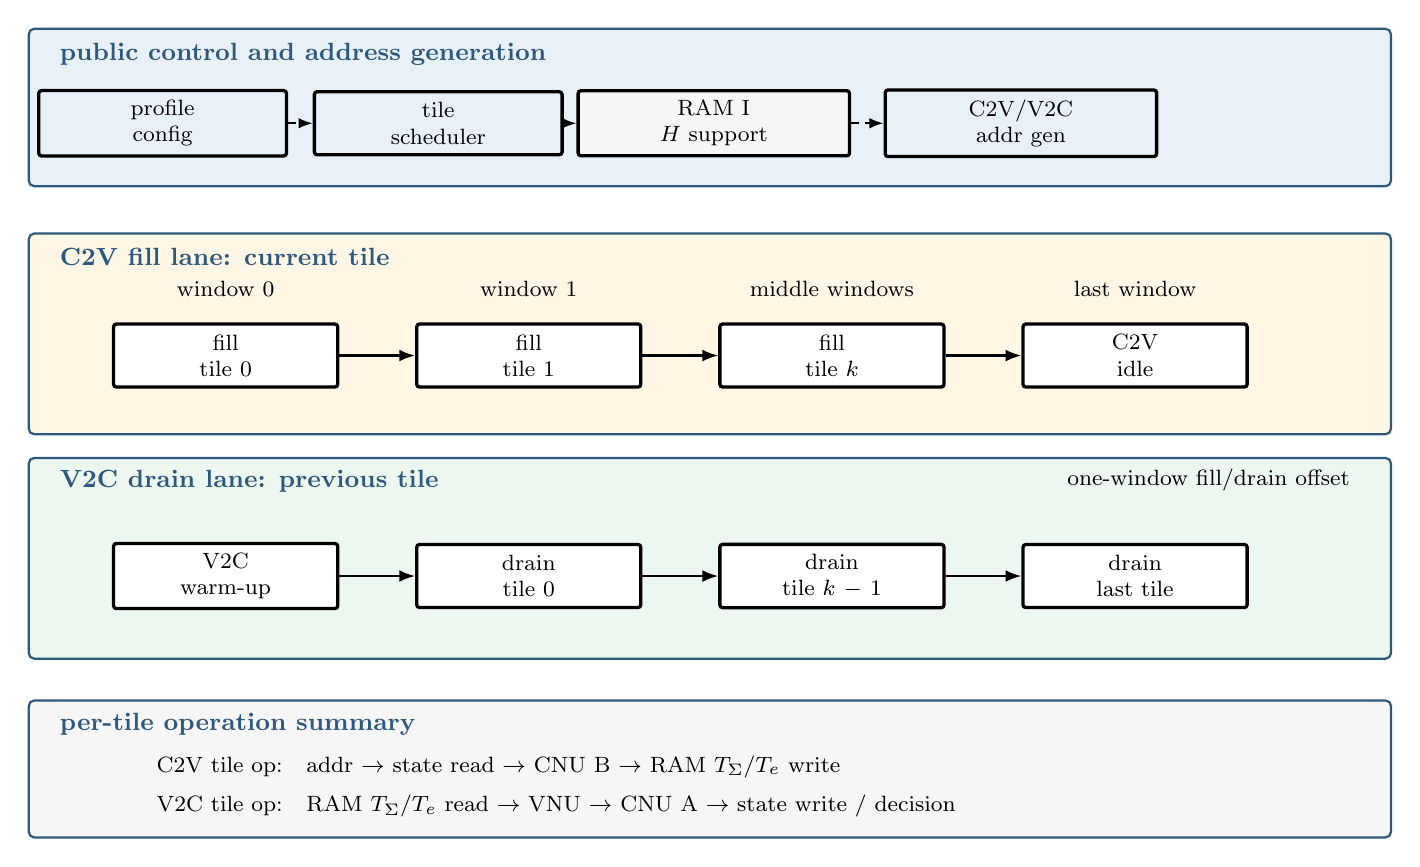
\begin{tikzpicture}[x=1cm,y=1cm]
    \begin{scope}[on background layer]
      \path[fill=ctrlfill, draw=accent, thick, rounded corners=2pt]
        (-0.45,8.45) rectangle (16.85,10.45);
      \path[fill=c2vfill, draw=accent, thick, rounded corners=2pt]
        (-0.45,5.30) rectangle (16.85,7.85);
      \path[fill=v2cfill, draw=accent, thick, rounded corners=2pt]
        (-0.45,2.45) rectangle (16.85,5.00);
      \path[fill=memfill, draw=accent, thick, rounded corners=2pt]
        (-0.45,0.18) rectangle (16.85,1.92);
    \end{scope}

    \node[title, anchor=west] at (-0.18,10.12) {public control and address generation};
    \node[title, anchor=west] at (-0.18,7.55) {C2V fill lane: current tile};
    \node[title, anchor=west] at (-0.18,4.70) {V2C drain lane: previous tile};
    \node[title, anchor=west] at (-0.18,1.62) {per-tile operation summary};

    \node[ctrl] (profile) at (1.25,9.25) {profile\\config};
    \node[ctrl] (sched) at (4.75,9.25) {tile\\scheduler};
    \node[mem] (rami) at (8.25,9.25) {RAM I\\$H$ support};
    \node[ctrl, text width=32mm] (addrgen) at (12.15,9.25) {C2V/V2C\\addr gen};

    \node[note] (time0) at (2.05,7.15) {window 0};
    \node[note] (time1) at (5.90,7.15) {window 1};
    \node[note] (timek) at (9.75,7.15) {middle windows};
    \node[note] (timel) at (13.60,7.15) {last window};

    \node[block, fill=white, text width=26mm] (c2v0) at (2.05,6.30) {fill\\tile 0};
    \node[block, fill=white, text width=26mm] (c2v1) at (5.90,6.30) {fill\\tile 1};
    \node[block, fill=white, text width=26mm] (c2vk) at (9.75,6.30) {fill\\tile $k$};
    \node[block, fill=white, text width=26mm] (c2vl) at (13.60,6.30) {C2V\\idle};

    \node[block, fill=white, text width=26mm] (v2c0) at (2.05,3.50) {V2C\\warm-up};
    \node[block, fill=white, text width=26mm] (v2c1) at (5.90,3.50) {drain\\tile 0};
    \node[block, fill=white, text width=26mm] (v2ck) at (9.75,3.50) {drain\\tile $k-1$};
    \node[block, fill=white, text width=26mm] (v2cl) at (13.60,3.50) {drain\\last tile};
    \node[note, anchor=east] at (16.45,4.72) {one-window fill/drain offset};

    \node[note, align=left, anchor=west] at (1.05,1.08) {C2V tile op:\quad
      addr $\rightarrow$ state read $\rightarrow$ CNU B $\rightarrow$ RAM $T_\Sigma/T_e$ write};
    \node[note, align=left, anchor=west] at (1.05,0.58) {V2C tile op:\quad
      RAM $T_\Sigma/T_e$ read $\rightarrow$ VNU $\rightarrow$ CNU A $\rightarrow$ state write / decision};

    \draw[ctl] (profile) -- (sched);
    \draw[ctl] (sched) -- (rami);
    \draw[ctl] (rami) -- (addrgen);

    \draw[sig] (c2v0) -- (c2v1);
    \draw[sig] (c2v1) -- (c2vk);
    \draw[sig] (c2vk) -- (c2vl);
    \draw[sig] (v2c0) -- (v2c1);
    \draw[sig] (v2c1) -- (v2ck);
    \draw[sig] (v2ck) -- (v2cl);
  \end{tikzpicture}
  \caption{Fixed-window tile schedule of the BIKE min-sum decoder.}
  \label{fig:decoder-schedule}
\end{figure}
\end{landscape}
\clearpage

\ifPDFTeX
\section{Top-Level Hardware Architecture}

Figure~\ref{fig:decoder-arch} shows the module-level decoder datapath. It keeps
the key storage and processing modules from \texttt{rtl/decoder\_top.sv}; control
logic is represented only by labeled input lines.
\else
\section{顶层硬件架构图}

图~\ref{fig:decoder-arch} 给出模块级译码器数据通路。该图保留
\texttt{rtl/decoder\_top.sv} 中最关键的存储和计算模块；控制逻辑只用带标注的输入线表示。
\fi

\begin{landscape}
\begin{figure}[p]
  \centering
  \resizebox{0.93\linewidth}{!}{%
  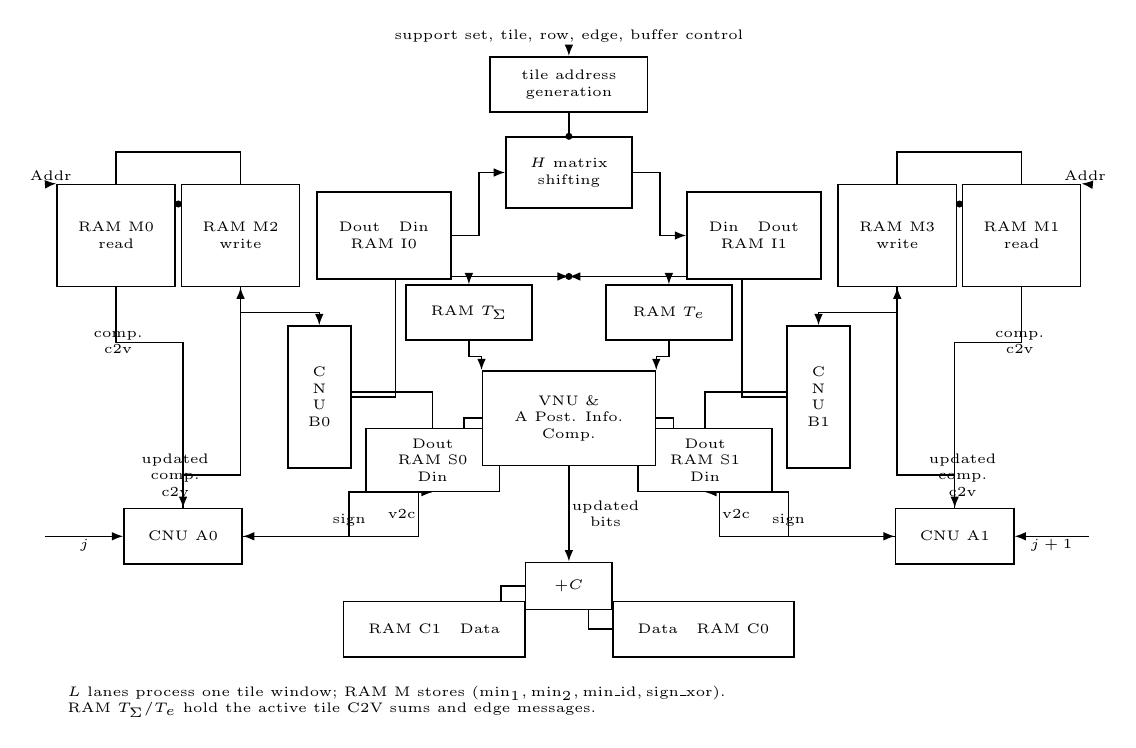
\begin{tikzpicture}[
      x=1cm,
      y=1cm,
      archbox/.style={
        draw,
        line width=0.55pt,
        fill=white,
        align=center,
        inner sep=1.5pt,
        minimum height=6.5mm,
        font=\tiny
      },
      ram/.style={archbox, minimum width=15mm, minimum height=13mm},
      smallram/.style={archbox, minimum width=17mm, minimum height=7mm},
      unit/.style={archbox, minimum width=16mm, minimum height=7mm},
      tallunit/.style={archbox, minimum width=8mm, minimum height=18mm},
      flow/.style={-{Latex[length=1.45mm,width=1.1mm]}, line width=0.55pt},
      wire/.style={line width=0.55pt},
      tap/.style={circle, fill=black, inner sep=0.9pt},
      label/.style={font=\tiny, inner sep=0.8pt, align=center}
    ]
    \node[ram] (m0) at (0.70,6.70) {RAM M0\\read};
    \node[ram] (m2) at (2.28,6.70) {RAM M2\\write};
    \node[smallram, minimum height=11mm] (i0) at (4.10,6.70)
      {Dout\quad Din\\RAM I0};
    \node[unit, minimum width=16mm, minimum height=9mm] (shift) at (6.45,7.50)
      {$H$ matrix\\shifting};
    \node[smallram, minimum height=11mm] (i1) at (8.80,6.70)
      {Din\quad Dout\\RAM I1};
    \node[ram] (m3) at (10.62,6.70) {RAM M3\\write};
    \node[ram] (m1) at (12.20,6.70) {RAM M1\\read};

    \node[tallunit] (b0) at (3.28,4.65) {C\\N\\U\\B0};
    \node[tallunit] (b1) at (9.62,4.65) {C\\N\\U\\B1};
    \node[smallram, minimum width=17mm, minimum height=8mm] (s0) at (4.72,3.85)
      {Dout\\RAM S0\\Din};
    \node[smallram, minimum width=17mm, minimum height=8mm] (s1) at (8.18,3.85)
      {Dout\\RAM S1\\Din};
    \node[unit, minimum width=22mm, minimum height=12mm] (vnu) at (6.45,4.38)
      {VNU \&\\A Post. Info.\\Comp.};

    \node[smallram, minimum width=16mm] (ts) at (5.18,5.72) {RAM $T_\Sigma$};
    \node[smallram, minimum width=16mm] (te) at (7.72,5.72) {RAM $T_e$};

    \node[unit, minimum width=15mm] (a0) at (1.55,2.88) {CNU A0};
    \node[unit, minimum width=15mm] (a1) at (11.35,2.88) {CNU A1};
    \node[smallram, minimum width=23mm] (c1) at (4.74,1.70)
      {RAM C1\quad Data};
    \node[smallram, minimum width=23mm] (c0) at (8.16,1.70)
      {Data\quad RAM C0};
    \node[unit, minimum width=11mm, minimum height=6mm] (gamma) at (6.45,2.25)
      {$+C$};

    \node[unit, minimum width=20mm, minimum height=7mm] (addr) at (6.45,8.62)
      {tile address\\generation};

    \begin{scope}[on background layer]
    \draw[flow] (6.45,9.08) -- (addr.north);
    \node[label, anchor=south] at (6.45,9.12)
      {support set, tile, row, edge, buffer control};
    \draw[flow] (i0.east) -- ++(0.35,0) |- (shift.west);
    \draw[flow] (shift.east) -- ++(0.35,0) |- (i1.west);
    \draw[wire] (addr.south) -- (shift.north);

    \draw[wire] (m0.north) -- ++(0,0.40) -| (m2.north);
    \draw[wire] (m3.north) -- ++(0,0.40) -| (m1.north);

    \draw[flow] (-0.20,7.35) -- node[label, above] {Addr} (m0.north west);
    \draw[flow] (13.05,7.35) -- node[label, above] {Addr} (m1.north east);
    \draw[flow] (-0.20,2.88) -- node[label, below] {$j$} (a0.west);
    \draw[flow] (13.05,2.88) -- node[label, below] {$j+1$} (a1.east);

    \draw[flow] (m2.south) -- ++(0,-0.32) -| (b0.north);
    \draw[flow] (m3.south) -- ++(0,-0.32) -| (b1.north);
    \draw[flow] (m0.south) -- ++(0,-0.70) -| node[label, pos=0.22, left]
      {comp.\\c2v} (a0.north);
    \draw[flow] (m1.south) -- ++(0,-0.70) -| node[label, pos=0.22, right]
      {comp.\\c2v} (a1.north);

    \draw[flow] (b0.east) -- (4.25,4.65) -- (4.25,6.18) -- (6.45,6.18);
    \draw[flow] (b1.west) -- (8.65,4.65) -- (8.65,6.18) -- (6.45,6.18);
    \draw[flow] (6.45,6.18) -- (5.18,6.18) -- (ts.north);
    \draw[flow] (6.45,6.18) -- (7.72,6.18) -- (te.north);
    \draw[flow] (ts.south) -- ++(0,-0.20) -| (vnu.north west);
    \draw[flow] (te.south) -- ++(0,-0.20) -| (vnu.north east);

    \draw[flow] (vnu.west) -- ++(-0.22,0) |- (s0.east);
    \draw[flow] (vnu.east) -- ++(0.22,0) |- (s1.west);
    \draw[flow] (vnu.south west) -- ++(-0.80,0) |- node[label, pos=0.34, left]
      {v2c} (a0.east);
    \draw[flow] (vnu.south east) -- ++(0.80,0) |- node[label, pos=0.34, right]
      {v2c} (a1.west);

    \draw[flow] (a0.north) -- ++(0,0.42) -| node[label, pos=0.25, left]
      {updated\\comp.\\c2v} (m2.south);
    \draw[flow] (a1.north) -- ++(0,0.42) -| node[label, pos=0.25, right]
      {updated\\comp.\\c2v} (m3.south);
    \draw[flow] (a0.east) -- ++(1.35,0) |- node[label, pos=0.28, below]
      {sign} (s0.south);
    \draw[flow] (a1.west) -- ++(-1.35,0) |- node[label, pos=0.28, below]
      {sign} (s1.south);
    \draw[flow] (s0.north) -- ++(0,0.45) -| (b0.south);
    \draw[flow] (s1.north) -- ++(0,0.45) -| (b1.south);

    \draw[flow] (vnu.south) -- node[label, right] {updated\\bits} (gamma.north);
    \draw[flow] (gamma.west) -- ++(-0.30,0) |- (c1.east);
    \draw[flow] (c0.west) -- ++(-0.30,0) |- (gamma.east);
    \end{scope}

    \node[tap] at (shift.north) {};
    \node[tap] at (1.49,7.10) {};
    \node[tap] at (11.41,7.10) {};
    \node[tap] at (6.45,6.18) {};

    \node[label, anchor=west, align=left] at (0.05,0.78)
      {$L$ lanes process one tile window; RAM M stores $(\min_1,\min_2,\mathrm{min\_id},\mathrm{sign\_xor})$.\\
       RAM $T_\Sigma/T_e$ hold the active tile C2V sums and edge messages.};
  \end{tikzpicture}
  }
  \caption{Top-level hardware architecture of the tile-based BIKE min-sum decoder.}
  \label{fig:decoder-arch}
\end{figure}
\end{landscape}
\clearpage

\begin{landscape}
\begin{figure}[p]
  \centering
  \resizebox{0.96\linewidth}{!}{%
  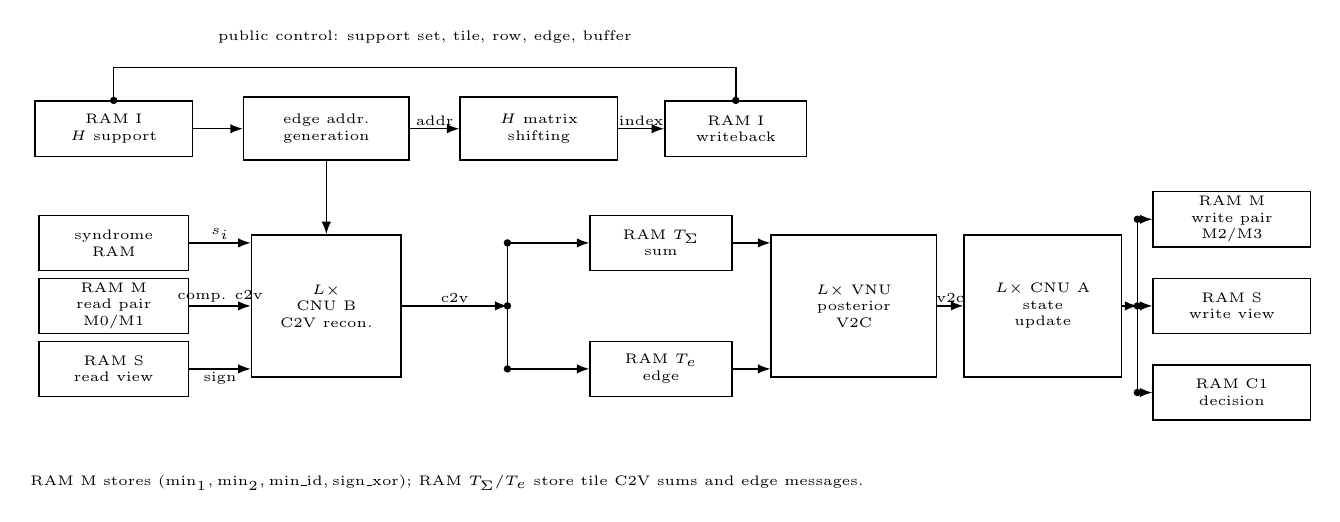
\begin{tikzpicture}[
      x=1cm,
      y=1cm,
      archbox/.style={
        draw,
        line width=0.55pt,
        fill=white,
        align=center,
        inner sep=1.6pt,
        minimum height=6.5mm,
        font=\tiny
      },
      mem/.style={archbox, minimum width=18mm, minimum height=7mm},
      proc/.style={archbox, minimum width=20mm, minimum height=8mm},
      tallproc/.style={archbox, minimum width=18mm, minimum height=18mm},
      flow/.style={-{Latex[length=1.6mm,width=1.2mm]}, line width=0.55pt},
      wire/.style={line width=0.55pt},
      tap/.style={circle, fill=black, inner sep=0.95pt},
      label/.style={font=\tiny, inner sep=1pt, align=center}
    ]
    \node[mem, minimum width=20mm] (rami) at (1.15,7.50) {RAM I\\$H$ support};
    \node[proc, minimum width=21mm] (addr) at (3.85,7.50) {edge addr.\\generation};
    \node[proc, minimum width=20mm] (shift) at (6.55,7.50) {$H$ matrix\\shifting};
    \node[mem, minimum width=18mm] (ramiwr) at (9.05,7.50) {RAM I\\writeback};

    \node[mem, minimum width=19mm] (synd) at (1.15,6.05) {syndrome\\RAM};
    \node[mem, minimum width=19mm] (mread) at (1.15,5.25) {RAM M\\read pair\\M0/M1};
    \node[mem, minimum width=19mm] (sread) at (1.15,4.45) {RAM S\\read view};

    \node[tallproc, minimum width=19mm] (cnub) at (3.85,5.25)
      {$L\times$\\CNU B\\C2V recon.};
    \node[mem, minimum width=18mm] (tsum) at (8.10,6.05) {RAM $T_\Sigma$\\sum};
    \node[mem, minimum width=18mm] (tedge) at (8.10,4.45) {RAM $T_e$\\edge};
    \node[tallproc, minimum width=21mm] (vnu) at (10.55,5.25)
      {$L\times$ VNU\\posterior\\V2C};
    \node[tallproc, minimum width=20mm] (cnua) at (12.95,5.25)
      {$L\times$ CNU A\\state\\update};

    \node[mem, minimum width=20mm] (mwrite) at (15.35,6.35)
      {RAM M\\write pair\\M2/M3};
    \node[mem, minimum width=20mm] (swrite) at (15.35,5.25)
      {RAM S\\write view};
    \node[mem, minimum width=20mm] (c1) at (15.35,4.15)
      {RAM C1\\decision};

    \coordinate (tbus) at (6.15,5.25);
    \coordinate (tbusTop) at (6.15,6.05);
    \coordinate (tbusBot) at (6.15,4.45);
    \coordinate (wbus) at (14.15,5.25);
    \coordinate (wbusTop) at (14.15,6.35);
    \coordinate (wbusBot) at (14.15,4.15);

    \node[label, anchor=south] at (5.10,8.55) {public control: support set, tile, row, edge, buffer};
    \draw[flow] (rami.east) -- (addr.west);
    \draw[flow] (addr.east) -- node[label, above] {addr} (shift.west);
    \draw[flow] (shift.east) -- node[label, above] {index} (ramiwr.west);
    \draw[wire] (ramiwr.north) -- ++(0,0.42) -| (rami.north);
    \node[tap] at (ramiwr.north) {};
    \node[tap] at (rami.north) {};
    \draw[flow] (addr.south) -- (cnub.north);

    \draw[flow] (synd.east) -- node[label, above] {$s_i$} (cnub.west |- synd.east);
    \draw[flow] (mread.east) -- node[label, above] {comp. c2v} (cnub.west);
    \draw[flow] (sread.east) -- node[label, below] {sign} (cnub.west |- sread.east);

    \draw[flow] (cnub.east) -- node[label, above] {c2v} (tbus);
    \node[tap] at (tbus) {};
    \draw[wire] (tbus) -- (tbusTop);
    \draw[wire] (tbus) -- (tbusBot);
    \node[tap] at (tbusTop) {};
    \node[tap] at (tbusBot) {};
    \draw[flow] (tbusTop) -- (tsum.west);
    \draw[flow] (tbusBot) -- (tedge.west);
    \draw[flow] (tsum.east) -- (vnu.west |- tsum.east);
    \draw[flow] (tedge.east) -- (vnu.west |- tedge.east);

    \draw[flow] (vnu.east) -- node[label, above] {v2c} (cnua.west);
    \draw[flow] (cnua.east) -- (wbus);
    \node[tap] at (wbus) {};
    \draw[wire] (wbus) -- (wbusTop);
    \draw[wire] (wbus) -- (wbusBot);
    \node[tap] at (wbusTop) {};
    \node[tap] at (wbusBot) {};
    \draw[flow] (wbusTop) -- (mwrite.west);
    \draw[flow] (wbus) -- (swrite.west);
    \draw[flow] (wbusBot) -- (c1.west);

    \node[label, anchor=west, align=left] at (0.05,3.00)
      {RAM M stores $(\min_1,\min_2,\mathrm{min\_id},\mathrm{sign\_xor})$; RAM $T_\Sigma/T_e$ store tile C2V sums and edge messages.};
  \end{tikzpicture}
  }
  \caption{Orthogonal datapath view of the tile-based BIKE min-sum decoder.}
  \label{fig:decoder-arch-orthogonal}
\end{figure}
\end{landscape}
\clearpage

\ifPDFTeX
\section{Architecture Description}

\subsection{Schedule Notation}

The figure is a schedule view. Each column is one fixed tile window. Window 0
primes the tile buffer, middle windows overlap C2V fill for tile $k$ with V2C
drain for tile $k-1$, and the last window drains the final tile. The operation
summary names the per-tile datapath stages: ``state read'' and ``state write''
are access views of the same RAM M/RAM S storage, while RAM $T_\Sigma$/RAM
$T_e$ provides the fill and active views of the tile buffer.
RAM M stores the compressed check state
$(\min_1,\min_2,\text{min\_id},\text{sign\_xor})$. RAM S stores the V2C sign
bits used by CNU B. RAM $T_\Sigma$ stores per-tile raw C2V sums, and RAM $T_e$
stores the per-edge C2V values needed by the V2C exclusion rule. CNU B
reconstructs C2V messages; VNU performs posterior and V2C updates; CNU A writes
the next compressed check state.

\subsection{Top-Level Organization}

The decoder receives a syndrome vector and the first-column support set of each
QC-MDPC circulant block. \texttt{ram\_i} stores the $N_0\times W$ base rows, and
\texttt{ram\_syndrome} stores the $r$ syndrome bits. In the unified build,
\texttt{decoder\_profile\_config} selects the public profile and emits $R$, $W$,
the tile count, row-bank depth, $C$, and the two shifts used to implement
$\alpha$. The main schedule is generated by \texttt{tile\_scheduler}, so the
decode order depends only on public parameters.

Local variable columns are grouped into tiles:
\[
  C_{\rm tile}=\min(R,\text{\texttt{BIKE\_C\_TILE}}),\quad
  Q_{\rm base}=\left\lceil\frac{C_{\rm tile}}{L}\right\rceil,\quad
  Q_{\rm tile}=Q_{\rm base}+3 .
\]
For every tile, every first-column support entry, and every \texttt{q\_seq},
\texttt{edge\_addr\_gen} expands the base row into the actual row, variable
column, edge id, row bank, and tile offset. The fixed guard cycles cover the
wrap split when the cyclic row index crosses $R-1\rightarrow 0$.

\subsection{C2V Pipeline}

The C2V path reconstructs check-to-variable messages from compressed check
state. Each active lane reads:
\[
  \text{RAM M}: (\min_1,\min_2,\text{min\_id},\text{sign\_xor}),\quad
  \text{RAM S}: \text{sign}(u_{i,j}),\quad
  \text{syndrome}: s_i .
\]
\texttt{cnu\_b} chooses \texttt{min1} or \texttt{min2} according to
\texttt{edge\_id} and computes
\[
  \text{sign}(v_{i,j})=\text{sign\_xor}\oplus \text{sign}(u_{i,j})\oplus s_i .
\]
The sign-magnitude C2V output is converted to a raw two's-complement value.
\texttt{ram\_t\_accum} accumulates the raw C2V sum for the variable column, and
\texttt{ram\_t} caches the individual edge message used by the V2C exclusion
rule. When \texttt{one\_idx==0}, the accumulator base for the variable column is
zero.

\subsection{V2C Pipeline}

The V2C path drains the previous tile from \texttt{ram\_t\_accum} and
\texttt{ram\_t}. \texttt{vnu\_update} computes, per lane,
\[
  \tilde\gamma_j = C + \alpha\sum_{i\in\mathcal{N}(j)} v_{i,j},
  \qquad
  u_{i,j}=C+\alpha\left(\sum_{i'\in\mathcal{N}(j)}v_{i',j}-v_{i,j}\right).
\]
Here $\alpha=2^{-s_0}+2^{-s_1}$ is implemented with shifts and addition in a
fixed-point fractional domain, followed by rounding back to an integer.
The V2C value is saturated into sign-magnitude form and sent to \texttt{cnu\_a}.
\texttt{cnu\_a} updates \texttt{min1}, \texttt{min2}, \texttt{min\_id}, and
\texttt{sign\_xor}; the compressed state is written to the \texttt{ram\_m}
write pair, and the V2C sign is written to \texttt{ram\_s}. On the final
iteration, the posterior sign is written to \texttt{ram\_c1} when
\texttt{one\_idx==0}.

\subsection{Storage and Double Buffering}

\texttt{ram\_m} is banked compressed check-state storage with two iteration
pairs. C2V reads the pair formed by the previous iteration, while V2C writes the
pair being formed for the following iteration. \texttt{ram\_s} stores V2C sign
bits at tile-word granularity. \texttt{ram\_t\_accum} is the double-buffered raw
C2V-sum storage used by the C2V read-accumulate-write path and the V2C sum
read. \texttt{ram\_t} is the double-buffered single-edge C2V cache.
\texttt{ram\_c1} stores the final error estimate.

The tile buffers alternate between \texttt{fill\_buf} and \texttt{active\_buf}.
Window 0 fills tile 0, middle windows run C2V on the current tile while V2C
drains the previous tile, and the last window drains the final tile.

\subsection{Fixed-Time Budget}

Each iteration first initializes the compressed check-state write pair:
\[
  T_{\rm clear}=\left\lceil\frac{R}{L}\right\rceil .
\]
Each tile window takes
\[
  T_{\rm tile}=W\cdot Q_{\rm tile}.
\]
With $T_{\rm total}=N_0\left\lceil R/C_{\rm tile}\right\rceil$, the iteration
latency and full decode latency are
\[
  T_{\rm iter}=T_{\rm clear}+(T_{\rm total}+1)\cdot T_{\rm tile},
  \qquad
  T_{\rm decode}=I_{\max}\cdot T_{\rm iter}.
\]
These quantities depend on the public profile, $L$, and $C_{\rm tile}$. The H
base rows, syndrome, error pattern, and convergence behavior affect only data
values, lane masks, or row addresses, not the number of main decode windows.
\else
\section{架构说明}

\subsection{调度图简写说明}

图中每一列表示一个固定 tile window。window 0 用来填充第一个 tile buffer；中间窗口将
tile $k$ 的 C2V 填充与 tile $k-1$ 的 V2C 排空重叠执行；最后一个窗口排空末尾 tile。
下方 operation summary 给出每个 tile 内部的数据通路阶段：state read 和 state write 是同一组
RAM M/RAM S 在 C2V 与 V2C 阶段的访问视图；RAM $T_\Sigma$/RAM $T_e$ 提供 tile buffer 的
fill/active 双缓冲视图。RAM M 表示压缩 check state 存储，内容为
$(\min_1,\min_2,\text{min\_id},\text{sign\_xor})$。RAM S 存储 CNU B 重建
C2V 时需要的 V2C 符号。RAM $T_\Sigma$ 存储 tile 内 raw C2V 总和，RAM $T_e$
存储排除自身时要减去的单边 C2V。CNU B 负责重建 C2V，VNU 负责 posterior 和 V2C
变量节点更新，CNU A 负责写入下一轮压缩 check state。

\subsection{顶层组织}

译码器输入为 syndrome 和 QC-MDPC 校验矩阵每个 circulant block 的第一列支撑集。\texttt{ram\_i}
保存 $N_0\times W$ 个 base row，\texttt{ram\_syndrome} 保存 $r$ 位 syndrome。统一参数配置下，
\texttt{decoder\_profile\_config} 根据公开 profile 输出 $R$、$W$、tile 数、row bank 深度、$C$ 和
$\alpha$ 的两个移位量。主译码由 \texttt{tile\_scheduler} 驱动，调度顺序只依赖公开参数。

局部变量列按 tile 组织：
\[
  C_{\rm tile}=\min(R,\text{\texttt{BIKE\_C\_TILE}}),\quad
  Q_{\rm base}=\left\lceil\frac{C_{\rm tile}}{L}\right\rceil,\quad
  Q_{\rm tile}=Q_{\rm base}+3 .
\]
调度器对每个 tile、每个第一列支撑项 \texttt{one\_idx}、每个 \texttt{q\_seq} 执行固定窗口。\texttt{edge\_addr\_gen}
把 base row、tile index 和 lane index 展开为实际 row、变量列、edge id、row bank 和 tile offset。
当循环行号跨越 $R-1\rightarrow 0$ 时，guard 周期承载固定的 micro-cycle 拆分。

\subsection{C2V 流水}

C2V 路径从压缩 check state 重建校验节点到变量节点的消息。每个有效 lane 读取：

\[
  \text{RAM M}: (\min_1,\min_2,\text{min\_id},\text{sign\_xor}),\quad
  \text{RAM S}: \text{sign}(u_{i,j}),\quad
  \text{syndrome}: s_i .
\]

\texttt{cnu\_b} 根据 \texttt{edge\_id} 选择 \texttt{min1} 或 \texttt{min2}，并计算
\[
  \text{sign}(v_{i,j})=\text{sign\_xor}\oplus \text{sign}(u_{i,j})\oplus s_i .
\]
输出的 sign-magnitude C2V 被转换为 two's complement 原始值。该值写入两个 tile buffer：
\texttt{ram\_t\_accum} 累加同一变量列收到的 raw C2V 总和，\texttt{ram\_t} 保存单条边的 raw C2V 消息。
\texttt{one\_idx==0} 的访问把该变量列的累加基值视为 0。

\subsection{V2C 流水}

V2C 路径读取前一个 tile 的 \texttt{ram\_t\_accum} 和 \texttt{ram\_t}。\texttt{vnu\_update} 在每 lane 计算：
\[
  \tilde\gamma_j = C + \alpha\sum_{i\in\mathcal{N}(j)} v_{i,j},
  \qquad
  u_{i,j}=C+\alpha\left(\sum_{i'\in\mathcal{N}(j)}v_{i',j}-v_{i,j}\right).
\]
其中 $\alpha=2^{-s_0}+2^{-s_1}$，RTL 通过两个左移到定点小数域后的加法实现，并在回到整数域时舍入。
V2C 结果饱和为 sign-magnitude 消息后送入 \texttt{cnu\_a}。\texttt{cnu\_a} 增量更新当前 row 的压缩状态：
符号进入 \texttt{sign\_xor}，幅度参与 \texttt{min1/min2/min\_id} 比较。更新后的状态写回 \texttt{ram\_m} 的 write pair，
V2C 符号写入 \texttt{ram\_s}，供后续 C2V 重建使用。最后一轮中，\texttt{one\_idx==0} 时 posterior 符号写入 \texttt{ram\_c1}
作为错误估计位。

\subsection{存储与双缓冲}

核心状态分为五类。\texttt{ram\_m} 是 banked compressed check-state storage，包含两个 pair；C2V 从 read pair
读取上一轮形成的状态，V2C 向 write pair 写入本轮形成的状态。\texttt{ram\_s} 存储每条 V2C 消息的符号位，
以 tile word 粒度读写。\texttt{ram\_t\_accum} 是 double-buffered raw C2V sum storage，服务于 C2V 的读-累加-写回
和 V2C 的求和读取。\texttt{ram\_t} 是 double-buffered edge cache，保存排除自身时需要减去的单条 C2V。
\texttt{ram\_c1} 保存最终错误估计并提供外部读口。

tile buffer 使用 \texttt{fill\_buf} 和 \texttt{active\_buf} 交替选择。第 0 个窗口只填充 tile 0；中间窗口让 C2V 处理当前 tile、
V2C 处理前一个 tile；最后一个窗口排空末尾 tile。该组织让每轮迭代包含固定的初始化和窗口数量。

\subsection{固定时间预算}

每轮先初始化 write pair 的压缩 check state，周期数为
\[
  T_{\rm clear}=\left\lceil\frac{R}{L}\right\rceil .
\]
每个 tile 窗口周期数为
\[
  T_{\rm tile}=W\cdot Q_{\rm tile}.
\]
总 tile 数为 $T_{\rm total}=N_0\left\lceil R/C_{\rm tile}\right\rceil$，每轮译码周期为
\[
  T_{\rm iter}=T_{\rm clear}+(T_{\rm total}+1)\cdot T_{\rm tile},
\]
完整译码周期为
\[
  T_{\rm decode}=I_{\max}\cdot T_{\rm iter}.
\]
这些量由公开 profile、$L$ 和 $C_{\rm tile}$ 决定。H 的 base row、syndrome、错误模式和收敛行为只影响数据值、
lane mask 或 row 地址，不改变主译码窗口数量。
\fi

\begin{thebibliography}{1}
\bibitem{cai2023}
J. Cai and X. Zhang, ``Low-complexity parallel min-sum medium-density parity-check decoder for McEliece cryptosystem,''
\emph{IEEE Transactions on Circuits and Systems I: Regular Papers}, vol. 70, no. 12, pp. 5327--5339, Dec. 2023.
\end{thebibliography}

\end{document}
